% id: 0493
% book: RPM 중3-2 수학 · 04 원주각
% section: 유형 20 두 원에서 접선과 현이 이루는 각
% figure: crop:fig-0493.png
% answer: ④
% answer_source: 답지
% variant_level: 0 (원본 전사)
% 이 파일은 build.mjs 가 items.json 에서 만든다. 고칠 때는 items.json 을 고친다.
다음 중 $\seg{AB}$와 $\seg{CD}$가 서로 평행하다고 할 수 \underline{없는} 것은?
\par\smallskip\begin{center}\setlength{\dmfigw}{215.2pt}\ifdim\dmfigw>\linewidth\setlength{\dmfigw}{\linewidth}\fi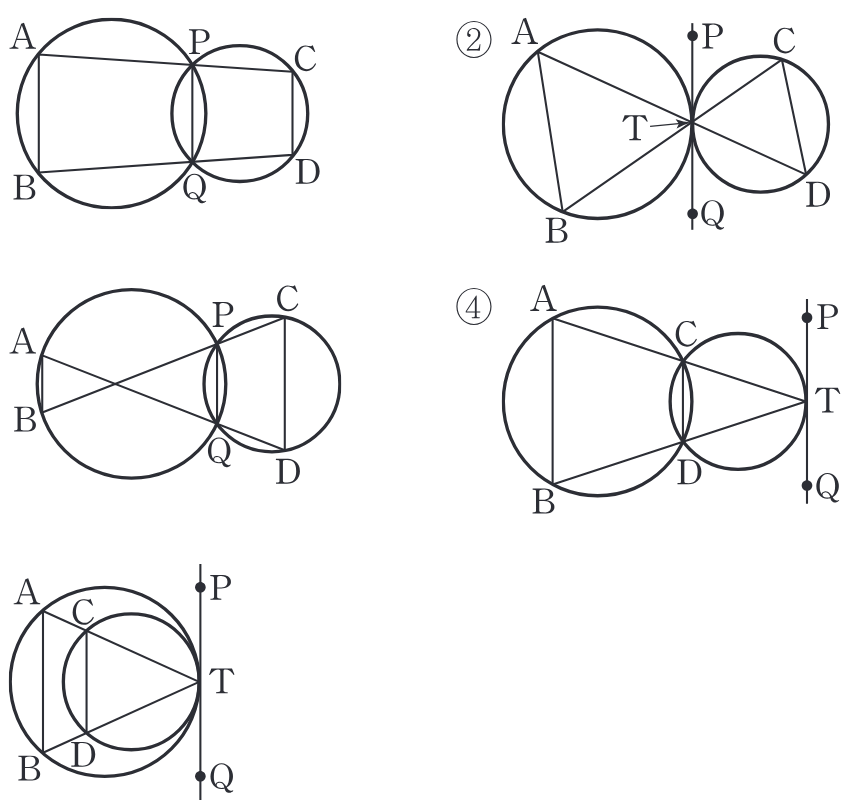
\includegraphics[width=\dmfigw]{figures/fig-0493.png}\end{center}
